\chapter{Vehicle Operating Cost Impacts}
\section{Introduction}
Vehicle costs are direct expenses that comprise the costs of vehicle ownership (fixed) and vehicle operation (variable). The latter category, typically referred to as vehicle operating costs (VOCs), varies with vehicle use and is typically expressed in cents per mile traveled by a vehicle. For most transportation modes, VOC involves energy use, tires, maintenance, repairs, and mileage-dependent depreciation. Fixed vehicle costs are those that are largely independent of vehicle use and are generally unaffected by transportation improvements; examples are insurance costs, time-dependent depreciation, financing, and storage. Such costs are therefore typically excluded from VOC impact evaluation of projects.\\\\
VOC savings or benefits of a transportation improvement or intervention simply refer to the reduction in vehicle operating costs compared to an existing situation or a base-case alternative.\\\\
For areawide or corridor-level projects involving multimodal systems, an improvement in any part of the system can affect VOCs of the other parts or other modes. For example, service improvement in commuter rail or provision of a bus rapid transit along a corridor can affect the level of service on highway facilities in the same corridor because the shift of some travelers from automobile to transit would lead to improved highway level of service due to reduced congestion and thus, lower vehicle operating costs at the highway section.\\\\
In this chapter we identify VOC components and factors and present a procedural framework for assessing the
VOC impacts of transportation improvements.
%%
\section{Components of Vehicle Operating Cost}
The components of vehicle operating cost are the individual items associated with vehicle operation on which expenses are directly incurred. These include the costs of energy needed to propel the vehicle, fluids, and other light consumables associated with mechanical working of the drivetrain, occasional replacement of the vehicle’s contact surfaces with the guideway, vehicle repair and maintenance, and vehicle depreciation.
\subsection{Fuel}
Fuel is a key component of vehicle operating costs. For highway vehicles for instance, fuel costs can account for 50 to 75\% of usage-related costs. Fuel cost can be estimated on the basis of fuel efficiency and unit fuel price. Fuel efficiency, in turn, depends primarily on vehicle class, type, age, and speed. Automobile associations, petroleum institutes, and government energy agencies publish fuel prices (dollars per gallon) on a regular basis. In the United States, the average prices of gasoline and diesel in 2005 were \$2.2 and \$2.4, respectively (USDOE, 2005b). Fuel prices for VOC computation purposes should be derived by subtracting the federal and state gasoline taxes from retail prices. On a mileage basis, the unit costs of fuel (including oil) in 2003–2004 ranged from approximately 7 cents per vehicle-mile for small autos to over 21 cents per vehicle-mile for large trucks (Barnes and Langworthy, 2003; AAA, 2005). Generally, very low speeds, steep uphill grades, and curves lead to higher fuel consumption rates and hence higher overall fuel costs. In the Highway Economic Requirements System (HERS) model (FHWA, 2002), the change in vehicle fuel efficiencies across the years is accounted for in VOC estimation using an adjustment factor.
%%
\subsection{Shipping Inventory}
The inventory cost of cargo (freight transportation) is a special category of user cost. The entity that ships the cargo (the client) is a user of a shipping service made available by a carrier. In the course of transporting perishable or valuable cargo, the client incurs holding costs that represent an opportunity cost: If at the beginning of the shipment, the client had a cash amount worth the cargo being shipped, such an amount would have earned some interest by the time the cargo reaches its destination. So by having the cargo transported, the client is foregoing some benefits. Higher inventory costs are generally directly related to cargo value, greater cargo perishability, higher prevailing opportunity cost of money, and slower speed of the shipping vehicle. To compute the inventory cost for a given vehicle class, an hourly discount rate is typically determined and multiplied by the average value of shipments undertaken by that vehicle class (FHWA, 2002). AASHTO (2003) recommends that the inventory costs of cargo per vehicle-mile should be applied to the unit user cost attributed to cargo-carrying transportation vehicles. The most significant VOC factors that affect the shipping inventory costs are speed and delay, but cargo value and interest rate also can be influential. Higher cargo value and interest rates and greater travel or transfer delay translate to higher unit costs of shipping inventory, and higher speeds lead to lower inventory costs. For example, at a 10\% interest rate, two trucks each shipping \$100,000 cargo, one traveling at 60 mph and the other at 50 mph, incur inventory costs of approximately 2.5 and 6 cents per mile, respectively (AASHTO, 2003).
%%
\subsection{Lubricating Oils for Mechanical Working of the Drivetrain}
The lubricating oil cost includes the cost of engine oil, transmission fluids, brake fluids, and other similar consumables associated with the operation of vehicle engine and drive train. Oil cost is a product of unit price (dollars/quart) and consumption rates (quarts/mile). The consumption rates depend on the amount of use as well as characteristics of the guideway and vehicle, and operational conditions such as speed, delay, grade, and curves. Typically, the cost of this set of VOC components is reported together with fuel costs, but some sources report them separately.
%%
\subsection{Preservation of the Vehicle-Guideway Contact Surface}
At their points of contact, both the vehicle and guideway experience deterioration due to wear and tear. For highways and runways, the vehicle contact is a tire; for railways, the contact is typically a steel wheel. Updated tire costs (2005 dollars) from the HERS technical report, are as follows: \$54.71 per tire for small autos, \$86.54 for medium-sized to large autos, \$95.39 for four-tire single-unit trucks, \$95.38 for sixtire single-unit trucks, \$230.10 for single-unit trucks of three or more axles, and \$569.74 for combination trucks. Of the various VOC factors, pavement condition, grade, curvature, and speed changes are those that most influence the rate of wear of contact surfaces.
%%
\section{Vehicle Repair and Maintenance}
Repair and maintenance costs are incurred on vehicle parts that need replacement or replenishment after some amount of use. For gasoline-powered vehicles, these include the cost of batteries, alternators, fuel pumps, air pump, tire rims, electrical parts such as bulbs and fuses, and so on. These costs also include costs of replacing parts due to crashes, misuse, or other adversarial factors. In some methodologies, the cost of vehicle repair and maintenance is not reported separately but is added to other nonfuel costs. In Year 2005 dollars, the unit cost of vehicle repair and maintenance generally ranged from 4.7 cents per vehicle-mile for small to medium-sized vehicles to 9.3 cents per vehicle-mile for trucks (AAA, 2005). Vehicle repair and maintenance are influenced by pavement condition, curvature, and to a lesser extent, speed, grade, and speed change.
%%
\subsection{Depreciation}
Vehicle depreciation is a function of vehicle usage (miles of travel) and vehicle age (years since manufacture). The table below presents the depreciation costs of selected vehicle classes and types. It can be seen that mileagebased depreciation rates are similar across vehicle classes: This seems reasonable because the lower initial cost of cars is balanced by their shorter service lives compared with trucks, so the net effect is that rates of mileage-based depreciation are similar across vehicle types (Barnes and Langworthy, 2003). Mileage-based depreciation costs can account for a significant fraction of overall vehicle operating costs. In some literature, the cost of vehicle depreciation is reported together with other nonfuel costs.
\begin{center}
	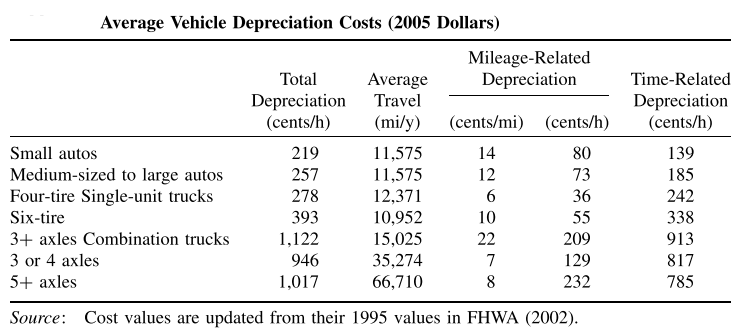
\includegraphics[scale=0.65]{gfx/fig63.png}
\end{center}
The values presented in the above table are average values. Depreciation rates actually vary by factors such as grade, curves, surface condition, and speed. An improvement in the transportation facility can produce a smoother pavement and improved driving conditions (through reduced stop-and-go situations). Also, all other factors remaining the same, increased speed can lead to reduced depreciation rates, as illustrated in the figure below, for straight constant-speed sections (FHWA, 2002).
\begin{center}
	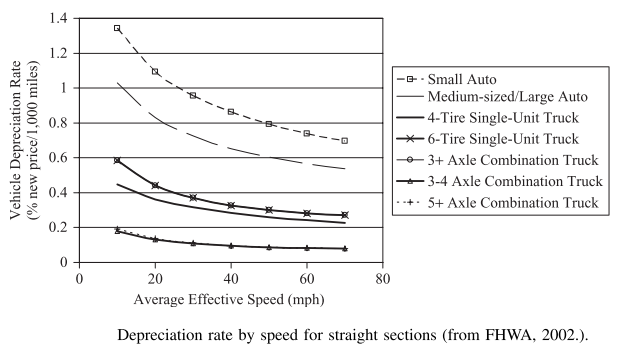
\includegraphics[scale=0.65]{gfx/fig64.png}
\end{center}
%%%%%
\section{Factors That Affect Vehicle Operating Cost}
For all modes of transportation, vehicle operating costs are affected by factors such as vehicle–operator characteristics, economic factors, condition and other characteristics of the fixed transportation facility, and policy–institutional factors. Although we focus on highway transportation in this section, the principles and concepts can be adapted to other transportation modes. The figure below shows the categories of highway VOC factors.
\begin{center}
	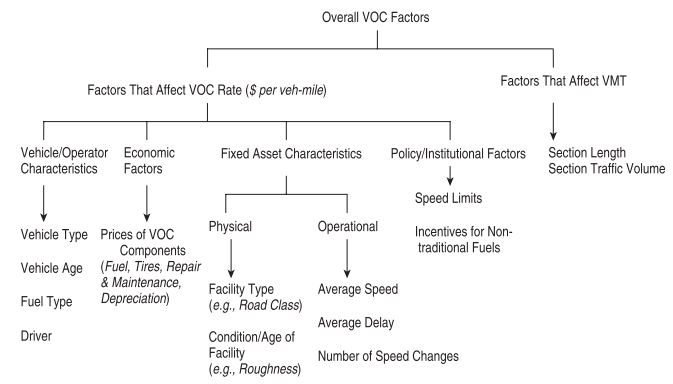
\includegraphics[scale=0.65]{gfx/fig65.png}
\end{center}
%%
\subsection{Vehicle Type}
Vehicle operating costs are influenced by size, class, and other vehicle characteristics. Trucks and buses generally have higher operating costs than automobiles, as they consume more fuel and oil and have higher prices for their vehicle parts. Even for a given vehicle type, there could be changes in VOC over time due to improved vehicle technology and fuel efficiency. If the analyst seeks to carry out long-term VOC impact evaluation, future levels of fuel efficiency could be extrapolated from past trends and duly factored in the VOC computation process.\\\\
In some cases, analysts may seek the operating costs associated with bicycling and walking to facilitate a more comprehensive comparison of transportation alternatives that include these modes. A standard bicycle with basic accessories can cost \$100 to \$500 with annualized maintenance costs of \$20 to \$40 for tire replacement, tire pumping, and security; for walking, the main consumable is that of footwear, which typically lasts 500 to 5000 miles of walking distance (VTPI, 2004). The human energy use associated with walking and cycling may be considered a benefit rather than a cost, particularly if traveling using these transportation modes substitute for other exercise activities.
%%
\subsection{Fuel Type}
The uncertainties in supply and increasing costs of fossil fuels coupled with their adverse environmental effects have led to growing use of alternative energy sources for transportation. In evaluating the impacts of transportation improvements, therefore, analysts need to account for the increasing percentage of alternative-fuel vehicles in the traffic stream. At the current time, electric and hybrid vehicles have relatively high purchase costs (150 to 200\% of the price of a comparable gasoline car). Electric cars require new battery sets every 20,000 to 30,000 miles costing \$2000 to \$3000 (averaging 6 to 15 cents per vehicle-mile), and consume 0.25 to 0.5 kWh per mile, so energy costs average 2 to 5 cents per kWh based on typical residential energy rates (USDOE, 2005a). The maintenance costs, including battery replacements, are significantly higher for electric cars (over four fold) compared to hybrid or conventional cars (VTPI, 2005). Even with traditional fuels, there are differences in cost across fuel types: in 2005, the average price of diesel was approximately 10\% higher than that of regular leaded gasoline. Also, there are price differences across the three standard grades of gasoline.
%%
\subsection{Longitudinal Grade} 
Uphill movements impose additional loads on vehicle engines and therefore require greater consumption of energy compared to downhill or level movements. For downhill trips, fuel consumption is lower than for uphill or level trips, but increased brake applications may lead to increased wear and tear of brake linings and therefore to increased cost of the brake maintenance component of VOC. The figure below illustrates the general relationships between grade and VOC at various speeds for medium-sized automobile. Generally, overall VOC is lowest for sections with gentle downward slopes (0 to -4\%).
\begin{center}
	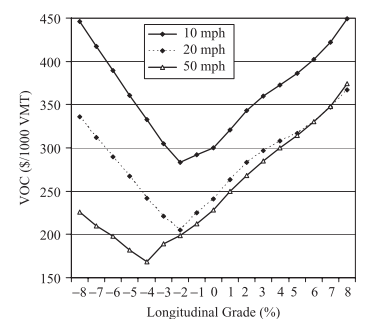
\includegraphics[scale=0.7]{gfx/fig66.png}
\end{center}
\textbf{\textit{Numerical Example:}}\\\\
A 2.15-mile section of State Road 25 on rolling terrain received major improvements in vertical alignment. The average grade of the section was reduced from 3.2\% to 2.5\%. Traffic volume and composition, and speed were the same after the improvement. Assume that the traffic stream has a 50:50 directional split and is composed primarily of medium-sized automobiles, and the traffic volume is 43,340 vpd (vehicles per day). In both cases, the average speed is 50 mph. What is the first year user benefit in terms of VOC?\\
\textit{Solution:}\\\\
Section Length (L) = 2.15 mile\\
Average Daily Traffic (ADT) = 43340 vpd\\
Average speed of the vehicle (v) = 50 mph\\\\
Before Improvement:\\
uphill: VOC at +3.2\% grade ($ {VOC}_1 $) = \$ 275/1000 VMT (using graph for medium-sized automobile)\\
downhill: VOC at -3.2\% grade ($ {VOC}_2 $) = \$ 190/1000 VMT (using graph for medium-sized automobile)\\
Average VOC before improvement ($ U_1 $) = $ \frac{275 + 190}{2} $ = \$232.5/1000 VMT\\
Vehicle Miles Travelled per year ($ {VMT}_1 $) = $ L \times ADT \times 360 = 2.15 \times 43340 \times 360 $ = 34011035 vehicle miles per year\\\\
After Improvement:\\
uphill: VOC at +2.5\% grade ($ {VOC}^{'}_1 $) = \$ 260/1000 VMT (using graph for medium-sized automobile)\\
downhill: VOC at -2.5\% grade ($ {VOC}^{'}_2 $) = \$ 200/1000 VMT (using graph for medium-sized automobile)\\
Average VOC after improvement ($ U_2 $) = $ \frac{260 + 200}{2} $ = \$230/1000 VMT\\
$ \because $ the traffic volume remains unchanged after improvement in longitudinal grade,\\
$ {VMT}_2 = {VMT}_1 $\\\\
Now,\\
Change in unit costs ($ U_1 - U_2 $) = 232.5 - 230 = 2.5/1000 VMT = 0.0025 VMT\\\\
$ \therefore $ First year user benefits = $ 0.5 \times (U_1 - U_2) \times ({VMT}_1 + {VMT}_2) $\\ = $ 0.5 \times 0.0025 \times 2 \times 34011065$ = \$ 85028
%%
\subsection{Vehicle Speed}
Vehicle operating speed is the dominant factor in determining VOC (Bennett, 1991; Thoresen and Roper, 1996; Bennett and Greenwood, 2001; FHWA, 2002). Transportation improvements influence travel speeds and therefore can profoundly affect VOC. For some vehicles, fuel consumption decreases with increasing speed to a certain point, after which there is little significant change (or sometimes, an increase) in fuel consumption with increasing speed. Factors that affect operating speeds, and subsequently influence fuel VOC, are speed limits (set by policy) and traffic conditions (which vary by the time of day—peak vs. nonpeak). In this section we discuss the impact of speed on shipping inventory costs and present some VOC models based on speed and other factors.
\subsubsection{a) Inventory Shipping}
Inventory cost is affected by vehicle speed and is calculated as follows:
\begin{equation}
	U_{IC} = 100 \times \frac{r}{365 \times 24} \times \frac{1}{S} \times P
\end{equation}
where $ U_{IC} $ is the user inventory cost in cents per vehicle mile, $ r $ the annual interest rate, $ P $ the cargo value in dollars, and $ S $ the vehicle speed in miles per hour.\\\\
\textbf{\textit{Numerical Example:}}\\
Due to a new speed limit policy, the average truck operating speed on a certain interstate freeway increased from 56.5 mph to 61.2 mph. Find the decrease in shipping inventory costs per year for trucks that comprise 22\% of the overall traffic stream of 82,500 vehicles per day (vpd). Each truck hauls an average of \$1.5 million worth of goods daily. Assume an 8\% interest rate.\\
\textit{Solution:}\\\\
The daily changes in inventory costs per truck due to the change in travel speed, $ \Delta U_{IC} $, can be estimated as follows:\\
$ \Delta U_{IC} = 100 \times \frac{r}{365 \times 24} \times \left( \frac{1}{S_0} - \frac{1}{S_1} \right) \times P$\\
$ 100 \times \frac{0.08}{365 \times 24} \times \left( \frac{1}{56.5} - \frac{1}{61.2} \right) \times 1500000 $\\
$ \therefore \Delta U_{IC} = 1.9178 $ cents/vehicle-mike\\\\
Then,\\
Number of trucks per year = (0.22)(82,500)(365) = 6,624,750\\
$ \therefore $ total reduction in inventory costs for all trucks per year = (1.9178/100)(6,624,750) = \$127,050 per mile
%%
\subsubsection{b) VOC Models and Look-up Table Based on Speed and Vehicle Class}
Hepburn (1994) developed a VOC model for urban roadways that considers the sum of four VOC components (tires, vehicle depreciation, maintenance, and fuel) as a function of two VOC factors: speed and vehicle class. The model is particularly useful for evaluating VOC impacts of transportation interventions that mostly yield a change in average operating speeds or policies that cause a shift in vehicle class distribution. The Hepburn function is as follows:\\\\
For “low” average travel: speeds ($ < $ 50 mph)
\begin{equation}
	VOC = C + \frac{D}{S}
\end{equation}
For “high” average travel: speeds ($ > $ 50 mph)
\begin{equation}
	VOC = a_0 - a_1 \times S + a_2 \times S^2
\end{equation}
where VOC is in cents/mile, $ S $ is speed (mph) and $ C $, $ D $, $ a_0 $, $ a_1 $,and $ a_2 $ are coefficients that are functions of vehicle class. The coefficient values are given in the table below:
\begin{center}
	\begin{tabular}{c c c c c c}
		Vehicle Type & $ C $ & $ D $ & $ a_0 $ & $ a_1 $ & $ a_2 $\\
		\hline
		small automobile & 24.8 & 45.5 & 27.2 & 0.035 & 0.00021\\
		medium-sized automobile & 28.5 & 95.3 & 33.5 & 0.058 & 0.00029\\
		large automobile & 29.8 & 163.4 & 38.1 & 0.093 & 0.00033
	\end{tabular}
\end{center}
The Hepburn model assumes that depreciation depends
entirely on vehicle use and that the depreciation rate is constant throughout vehicle life. Furthermore, the model is for tangent, level, and urban road sections with pavement roughness assumed to remain constant over time, and all VOC component costs assumed to vary with distance, with the exception of fuel cost, which varies with speed. It does not explicitly consider the consumption rates and prices of individual VOC components for each vehicle class but is nevertheless useful for quick estimation of VOC.\\\\
\textbf{\textit{Numerical Example:}}\\
A straight and level urban arterial has an average operating speed of 35 mph. What is the unit VOC of medium-sized automobiles that use this highway?\\
\textit{Solution:}\\\\
Knowing the values of C and D from Table:\\\\
$ VOC = C + \frac{D}{S} = 28.5 + \frac{95.3}{35} $ = 31.22 cents/vehicle-mile
\subsubsection{c) VOC model based on speed, grade, and vehicle class}
Zaniewski (1982) provided a VOC model as a function of speed, grade, and vehicle class. Table 7.4 presents the VOCs for medium-sized autos, with updated cost values. If the project section consists of several segments with different grades or VMTs, the unit VOC (dollars/vehicle-mile) is estimated separately for each segment. It should be noted, however, that the vehicles at the time of the Zaniewski study (ca. 1980) had 17\% lower fuel efficiency than vehicles in 1997 (FHWA, 2002), and even lower compared to vehicles in 2005. As such, Table given below should be used after stating the necessary assumptions regarding fuel efficiency, or after making due adjustments for fuel efficiency changes over the years.
\begin{center}
	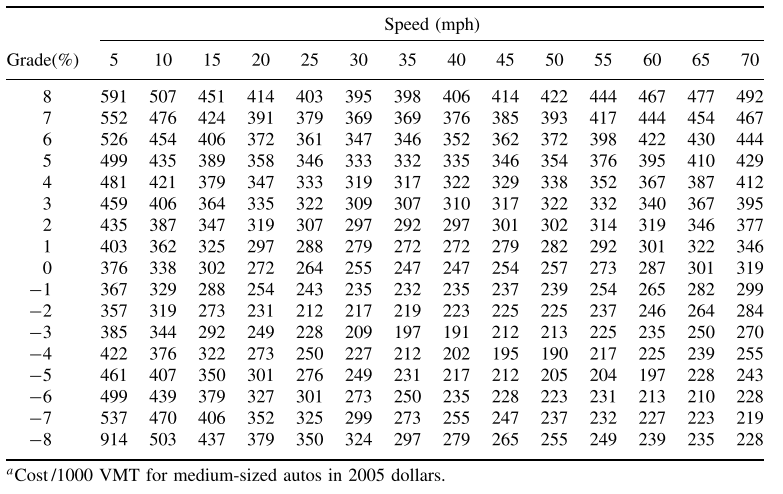
\includegraphics[scale=0.6]{gfx/fig67.png}
\end{center}